\chapter{Risultati}
\label{chap:risultati}

In questo capitolo vengono presentati e discussi i risultati delle due campagne
di misura descritte nel capitolo precedente. La \textbf{Campagna A} (dataset
intero, 2 thread, tre ripetizioni) fornisce il confronto tra i sei modelli su
efficienza energetica e qualità a parità di grado di parallelismo; la
\textbf{Campagna B} (stesso insieme di 150 prompt, thread 1, 2 e 4, singola
ripetizione) mette in luce l'effetto del grado di parallelismo su latenza, potenza
ed energia. Nella Campagna A i valori riportati sono la media sulle tre
ripetizioni; le grandezze energetiche sono espresse come \textit{energia netta per
inferenza} (Joule), al netto del consumo di base della scheda
(Equazione~\ref{eq:energia_netta}).

\section{Confronto tra i modelli (Campagna A)}

\subsection{Efficienza energetica}

La Figura~\ref{fig:res-energia} riporta l'energia netta media per inferenza di
ciascun modello, eseguito a 2 thread. Il modello più efficiente risulta
\textbf{qwen2.5-1.5B Q4\_K\_M} con circa \textbf{24,6~J} per inferenza, mentre il
più energivoro è \textbf{Llama-3.2-3B Q8\_0} con circa \textbf{64,0~J}, oltre due
volte e mezza. Confrontando ciascuna famiglia nelle due precisioni, le varianti a
8 bit (Q8\_0) consumano in media circa il \textbf{22\% in più} rispetto alle
corrispondenti a 4 bit (Q4\_K\_M) --- \mbox{+24\%} per gemma, \mbox{+28\%} per
llama, \mbox{+6\%} per qwen. A parità di modello, i pesi a 8 bit occupano più
memoria e richiedono di leggere più byte per ogni token generato: su un
dispositivo limitato dalla larghezza di banda della memoria come il Raspberry
Pi~5, questo si traduce direttamente in un consumo maggiore.

\begin{figure}[htbp]
    \centering
    
\includegraphics[width=\textwidth]{imm/efficiency_jpt.png}
    \caption{Energia netta media per inferenza dei sei modelli (Campagna A, 2 thread).}
    \label{fig:res-energia}
\end{figure}

Oltre all'energia per singola inferenza, la Figura~\ref{fig:res-energia-tot}
riporta l'energia complessiva spesa da ciascuna configurazione per completare
l'intera suite di benchmark: la più economica è \textbf{qwen2.5-1.5B Q4\_K\_M}
(circa \textbf{3700~J} per i 150 prompt), mentre la più dispendiosa è
\textbf{Llama-3.2-3B Q8\_0} (circa \textbf{9600~J}, oltre 2,5 volte tanto).
L'ordine ricalca quello dell'energia per inferenza, confermando qwen come il più
parsimonioso e llama come il più oneroso.

\begin{figure}[htbp]
    \centering
    
\includegraphics[width=\textwidth]{imm/energy_per_config.png}
    \caption{Energia totale consumata da ciascuna configurazione per completare la suite di benchmark (Campagna A, i sei modelli a 2 thread).}
    \label{fig:res-energia-tot}
\end{figure}

La \textbf{potenza media} assorbita durante l'inferenza è invece \emph{pressoché
costante} tra i modelli (circa \textbf{6,2~W} a 2 thread, entro un intervallo di
6,1--6,3~W, Figura~\ref{fig:res-potenza-modelli}): essa dipende essenzialmente dal
grado di utilizzo della CPU imposto dal livello di parallelismo, e non dalla
dimensione o dal livello di quantizzazione del modello. Ne consegue un'osservazione
importante: poiché l'energia è il prodotto della potenza per il tempo
($E = P \cdot \Delta t$) e la potenza è quasi la stessa per tutti, le differenze di
energia per inferenza osservate tra i modelli derivano quasi interamente dalla
diversa \textbf{durata} dell'inferenza (la latenza), più che da una diversa potenza
istantanea.

\begin{figure}[htbp]
    \centering
    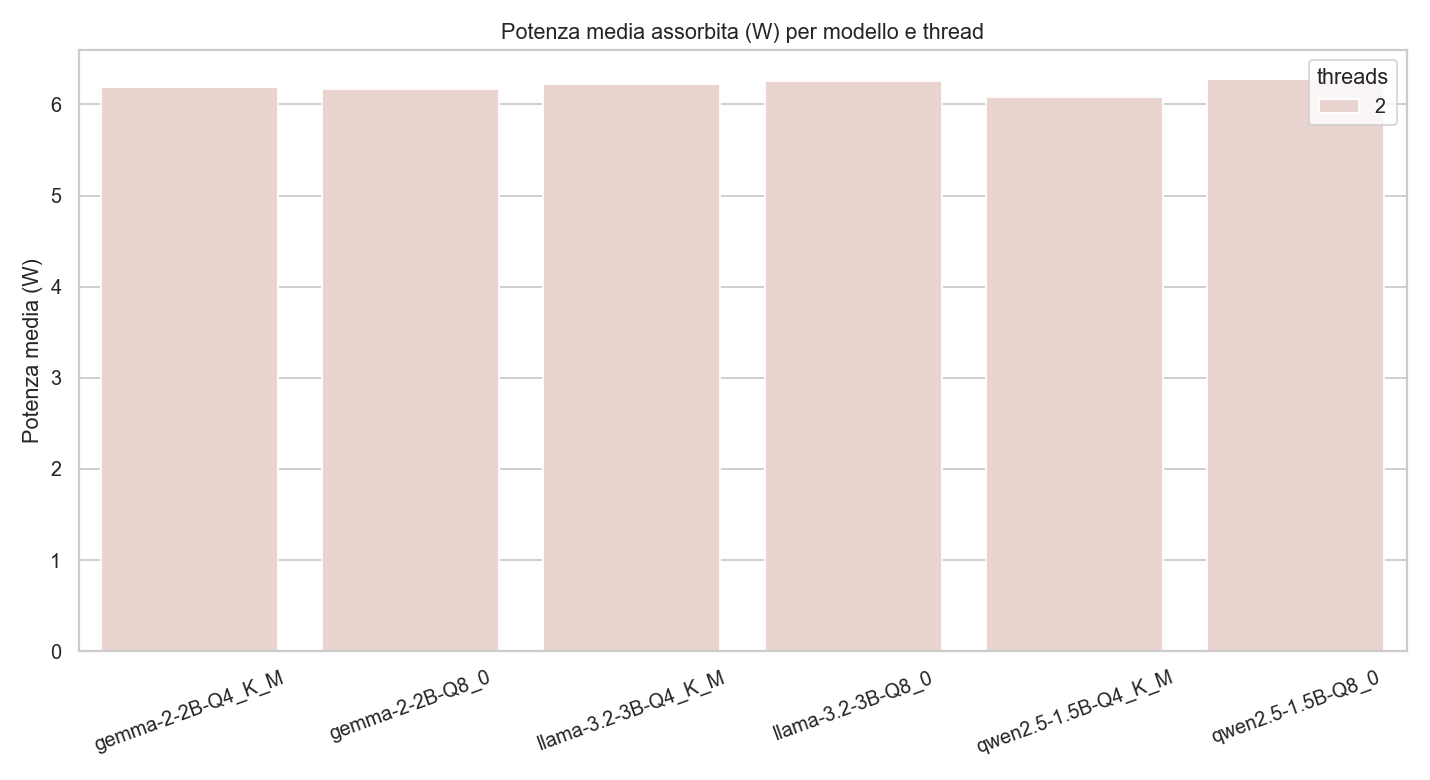
\includegraphics[width=\textwidth]{imm/power_a.png}
    \caption{Potenza media assorbita per modello, a 2 thread (Campagna A). La potenza
    è pressoché costante tra i modelli, poiché determinata dal grado di parallelismo
    più che dal modello eseguito.}
    \label{fig:res-potenza-modelli}
\end{figure}

\subsection{Qualità delle risposte}

La Figura~\ref{fig:res-qualita} mostra, sotto forma di mappa di calore, la
frazione di risposte corrette (score da 0 a 1) di ciascun modello su ciascun
benchmark. Il modello con la qualità media più elevata è \textbf{qwen2.5-1.5B
Q4\_K\_M} (accuratezza media circa \textbf{0,71}), mentre il valore più basso
spetta a \textbf{gemma-2-2B Q8\_0} (0,66); le differenze fra modelli restano
comunque contenute (tutti tra 0,66 e 0,71). A livello di singolo benchmark
emergono però specializzazioni marcate: il modello più grande, Llama-3.2-3B,
eccelle sui task di ragionamento --- BIG-Bench Hard (0,80) e GSM8K (fino a 0,80)
--- mentre i modelli più piccoli lo superano nettamente sui quesiti di senso
comune (CommonsenseQA, qwen fino a 0,77 contro circa 0,53 di llama) e sulla
generazione di codice (HumanEval, qwen fino a 0,84 contro 0,56 di llama); su
TruthfulQA i valori sono ravvicinati (gemma fino a 0,74). Riguardo all'effetto
della quantizzazione sulla qualità, il passaggio da 8 a 4 bit comporta una
differenza del tutto \textbf{trascurabile} (accuratezza media 0,68 a 8 bit contro
0,69 a 4 bit): la quantizzazione più aggressiva a 4 bit non degrada in pratica la
qualità delle risposte, pur dimezzando circa lo spazio occupato e riducendo
sensibilmente il consumo.

Occorre interpretare correttamente le differenze di accuratezza osservate a livello di
\emph{singolo benchmark}, che in alcuni casi appaiono ampie tra le due precisioni dello
stesso modello (ad esempio qwen2.5-1.5B su GSM8K: 0,57 a 4 bit contro 0,41 a 8 bit).
Esse derivano dalla combinazione di due fattori.

Il primo è che la quantizzazione produce modelli \emph{genuinamente diversi}:
arrotondando i pesi a 4 o a 8 bit si modificano leggermente le distribuzioni di
probabilità sui token. Sui prompt in cui il modello è "sicuro" il token più probabile
resta lo stesso e la risposta non cambia; sui prompt \emph{incerti}, invece, anche una
piccola perturbazione dei pesi può ribaltare l'esito. Le divergenze tra le due
precisioni si concentrano perciò sui compiti \textbf{al limite delle capacità del
modello} --- come il ragionamento aritmetico multi-passaggio di GSM8K per un modello da
appena 1,5 miliardi di parametri --- mentre sui compiti in cui il modello è a suo agio
le due precisioni coincidono quasi perfettamente (su CommonsenseQA, ad esempio,
qwen2.5-1.5B a 4 e a 8 bit ottiene risultati praticamente identici).

Il secondo fattore è che ciascun benchmark è valutato su soli \textbf{30 prompt}:
l'accuratezza di una singola cella porta quindi un'incertezza statistica dell'ordine di
$\pm 9$ punti percentuali (l'errore standard di una proporzione stimata su 30 campioni),
per cui uno scarto di cella anche ampio può non riflettere una reale differenza di
qualità. Per questi motivi la mappa di calore va letta come indicativa delle
\emph{tendenze} per singolo compito, mentre il confronto affidabile è quello condotto
sulla \textbf{media complessiva} dei 150 prompt (Figura~\ref{fig:res-qualita-media}): lì
gli intervalli di confidenza al 95\% delle due precisioni di ogni famiglia si
sovrappongono, e il verso stesso dello scarto cambia da famiglia a famiglia (8 bit
lievemente superiore per Llama-3.2-3B, 4 bit per gemma e qwen), a conferma che 4 e 8 bit
sono \textbf{sostanzialmente equivalenti} in qualità e che nessuna delle due precisioni
è sistematicamente migliore.

\begin{figure}[htbp]
    \centering
    
\includegraphics[width=\textwidth]{imm/quality_heatmap.png}
    \caption{Qualità delle risposte (accuratezza media) per modello e benchmark (Campagna A).}
    \label{fig:res-qualita}
\end{figure}

\begin{figure}[htbp]
    \centering
    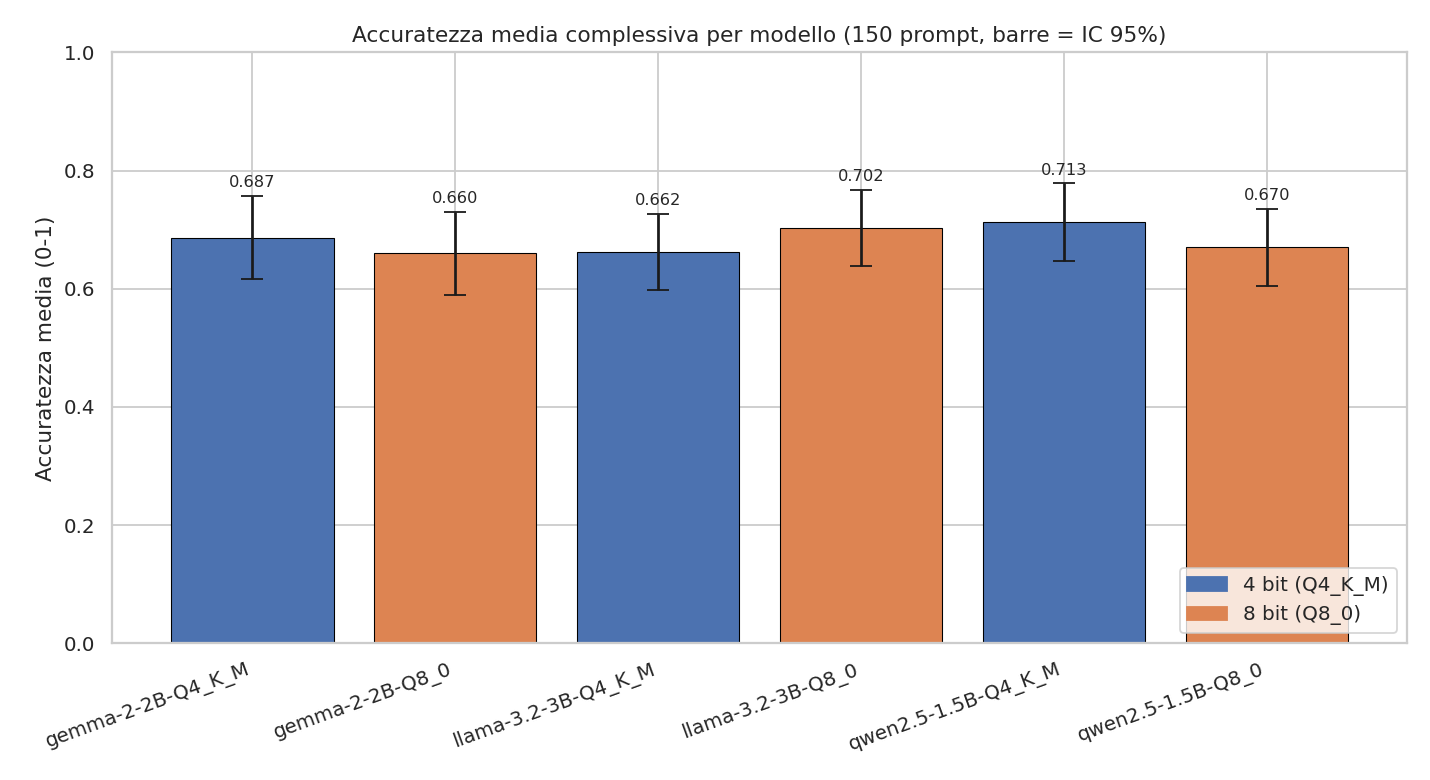
\includegraphics[width=\textwidth]{imm/quality_overall.png}
    \caption{Accuratezza media complessiva per modello (Campagna A, 150 prompt), con
    barre d'errore pari all'intervallo di confidenza al 95\%. All'interno di ogni
    famiglia gli intervalli delle due precisioni (4 e 8 bit) si sovrappongono
    ampiamente: le differenze di qualità non sono statisticamente significative.}
    \label{fig:res-qualita-media}
\end{figure}

\subsection{Velocità di elaborazione}

La Figura~\ref{fig:res-throughput} riporta la velocità di elaborazione dei prompt
(\textit{prompt processing}) e di generazione (\textit{generation}) in token al
secondo. La generazione, che determina in larga parte la latenza percepita, varia
da circa \textbf{5,1} a \textbf{17,9} token/s a seconda del modello: come atteso i
modelli più piccoli (qwen2.5-1.5B, fino a 17,9~t/s) generano molto più
rapidamente dei più grandi (Llama-3.2-3B e gemma-2-2B a 8 bit, intorno a
5,1~t/s). L'effetto della quantizzazione sulle due fasi è però \emph{opposto}. In
\textbf{generazione} --- che produce un token alla volta ed è limitata dalla
larghezza di banda della memoria --- il 4 bit è più veloce dell'8 bit (ad esempio
qwen2.5-1.5B: 17,9 contro 11,5~t/s), perché deve leggere circa metà dei byte per
token. Nel \textbf{prompt processing}, invece, i token del prompt vengono elaborati
insieme (prodotti matrice-matrice, con i pesi riutilizzati su molti token): la fase è
limitata dal \emph{calcolo} più che dalla memoria, e a pesare è il costo di
dequantizzazione dello schema a 4 bit (Q4\_K\_M, più complesso del semplice Q8\_0). Di
conseguenza è l'\textbf{8 bit} a risultare più veloce nel prompt processing
(qwen2.5-1.5B: 41,2 contro 31,8~t/s; gemma e Llama circa \mbox{+10--13\%}). Poiché
però la latenza complessiva è dominata dalla generazione (256 token prodotti a fronte
di prompt brevi), nel complesso il 4 bit resta più rapido \emph{end-to-end}.

Questo effetto si riflette direttamente sulla \textbf{latenza} di inferenza
(Figura~\ref{fig:res-latenza-modelli}). A parità
di modello e di parallelismo (2 thread), le varianti a \textbf{8 bit} risultano
mediamente circa il \textbf{30\% più lente} delle corrispondenti a 4 bit: l'aumento
va da \mbox{+13\%} per qwen2.5-1.5B (da 6,0 a 6,8~s) a \mbox{+34\%} per gemma-2-2B
(da 9,6 a 12,9~s) e \mbox{+37\%} per Llama-3.2-3B (da 12,1 a 16,5~s). La ragione è
la stessa che spiega il maggior consumo: gli 8 bit richiedono di leggere circa il
doppio dei byte per ogni token generato e, su un dispositivo limitato dalla larghezza
di banda della memoria, ciò allunga in proporzione i tempi di generazione. I 4 bit
offrono quindi, oltre a un minor consumo, anche una latenza sensibilmente inferiore.

\begin{figure}[htbp]
    \centering
    
\includegraphics[width=\textwidth]{imm/throughput.png}
    \caption{Velocità di elaborazione (prompt e generazione) per modello (Campagna A).}
    \label{fig:res-throughput}
\end{figure}

\begin{figure}[htbp]
    \centering
    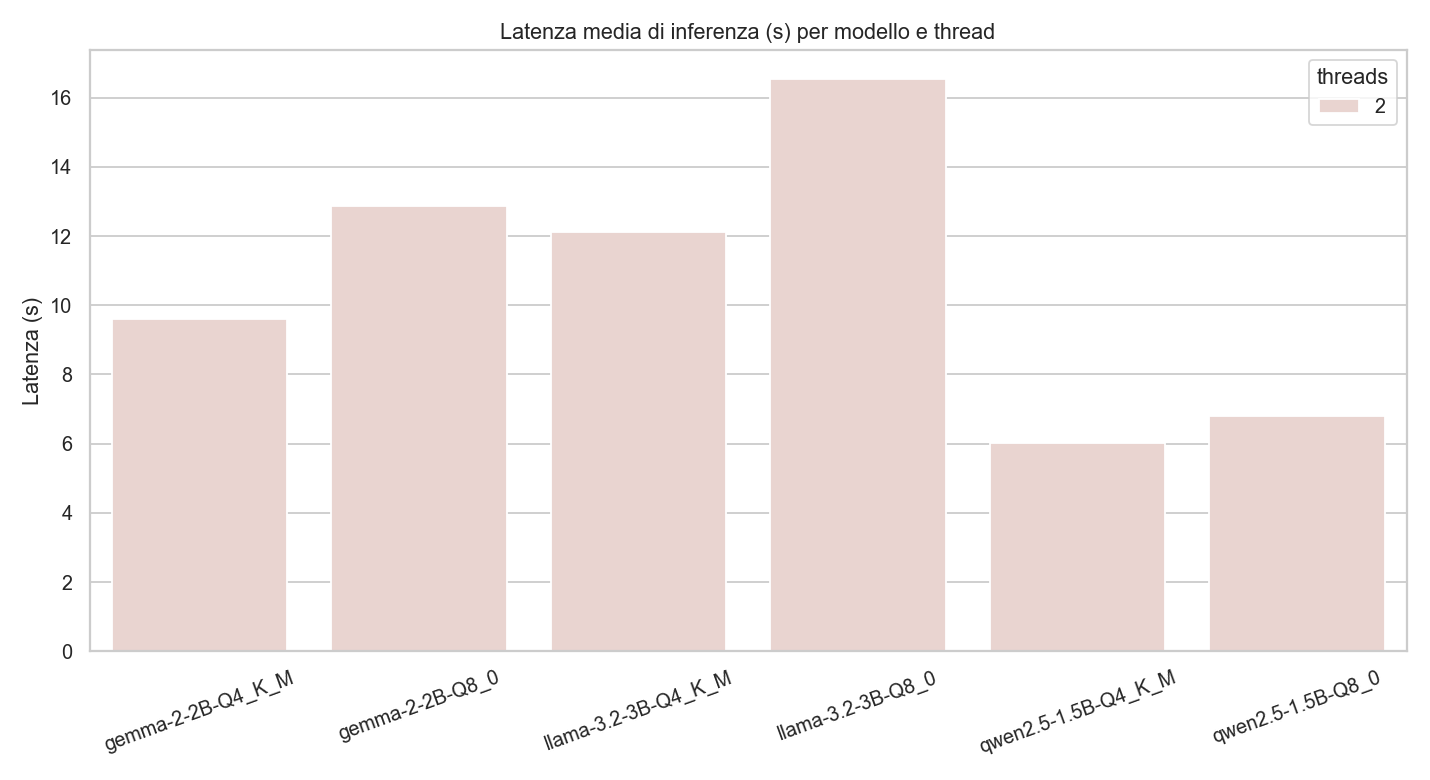
\includegraphics[width=\textwidth]{imm/latency_a.png}
    \caption{Latenza media di inferenza per modello, a 2 thread (Campagna A). A parità
    di famiglia, la variante a 8 bit (Q8\_0) presenta una latenza superiore rispetto a
    quella a 4 bit (Q4\_K\_M).}
    \label{fig:res-latenza-modelli}
\end{figure}

\section{Effetto del grado di parallelismo (Campagna B)}
\label{sec:camp-b}

Poiché il numero di thread influenza solo i tempi e i consumi dell'inferenza e
non le risposte generate dal modello, in questa campagna la qualità non viene
ridiscussa: essa è stata misurata in modo robusto nella Campagna A. Qui
l'attenzione è rivolta all'effetto del parallelismo su latenza, potenza ed
energia.

\subsection{Latenza}

La Figura~\ref{fig:res-latenza} mostra la latenza media di inferenza al variare
del numero di thread (1, 2 e 4). Passando da 1 a 2 thread la latenza si riduce di
circa \textbf{24\%} (da 14,2 a 10,9~s in media), mentre l'ulteriore passaggio da 2
a 4 thread non porta alcun guadagno --- anzi la latenza \emph{peggiora}
(circa \mbox{+18\%}, risalendo a 12,8~s). Diversi benchmark sono limitati dalla
larghezza di banda della memoria più che dal numero di core: il terzo e quarto core
non accelerano la generazione e introducono contesa. Il valore ottimale di
parallelismo risulta quindi \textbf{2 thread}.

Un dettaglio interessante riguarda il confronto tra le due precisioni \emph{a 1 thread}:
per ogni modello la latenza è più bassa con la variante a \textbf{8 bit} che con quella a
4 bit (ad esempio qwen2.5-1.5B: 7,6~s contro 9,6~s), in apparente contrasto con il fatto
che i 4 bit debbano leggere meno dati. La spiegazione è ancora la distinzione tra carico
limitato dalla \emph{memoria} e carico limitato dal \emph{calcolo}. Con un solo thread il
bus di memoria non è saturo, quindi anche la generazione è più \emph{compute-bound} che
\emph{memory-bound}: in questo regime il vantaggio del 4 bit (metà dei byte da leggere) è
annullato dal suo maggior costo di \textbf{dequantizzazione} (lo schema Q4\_K\_M è più
complesso del semplice Q8\_0), tanto che la velocità di generazione delle due precisioni
diventa praticamente identica (a 1 thread circa 7,7~t/s per il 4 bit contro 7,5~t/s per
l'8 bit). A ciò si aggiunge la fase di \emph{prompt processing}, anch'essa compute-bound e
più rapida a 8 bit: il risultato netto è una latenza complessiva inferiore per l'8 bit a
1 thread. Passando a 2 o 4 thread, invece, i core saturano la banda di memoria e la
generazione torna \emph{memory-bound}: il 4 bit riprende un netto vantaggio (a 2 thread
11,5 contro 7,4~t/s) e, poiché la generazione domina la latenza complessiva, è di nuovo
il 4 bit ad avere la latenza più bassa.

\begin{figure}[htbp]
    \centering
    
\includegraphics[width=\textwidth]{imm/latency.png}
    \caption{Latenza media di inferenza al variare del numero di thread (Campagna B).}
    \label{fig:res-latenza}
\end{figure}

\subsection{Potenza ed energia}

All'aumentare del numero di thread la potenza media assorbita \textbf{cresce}
(da circa 4,9~W a 1 thread a 7,0~W a 4 thread, Figura~\ref{fig:res-potenza}).
L'energia netta per inferenza è \textbf{minima a 1 thread} (circa 40,6~J) e cresce
con il parallelismo: solo lievemente da 1 a 2 thread (\mbox{+10\%}, circa 44,8~J),
ma nettamente a 4 thread (\mbox{+28\%} rispetto a 2 thread, circa 57,5~J). In
termini di sola energia il minimo si ha quindi a 1 thread, ma a fronte di una
latenza molto più elevata; il miglior compromesso tra \textit{time-to-answer} ed
efficienza energetica è a \textbf{2 thread}, che riduce di circa un quarto la
latenza con un modesto sovrapprezzo energetico, mentre a 4 thread si perde su
entrambi i fronti.

Un dettaglio degno di nota riguarda il confronto tra le due precisioni al variare del
parallelismo: la potenza media delle varianti a 4 e a 8 bit si \emph{ribalta} passando
da 1 a 4 thread. A \textbf{1 thread} le varianti a 8 bit assorbono circa 0,4~W in più
delle corrispondenti a 4 bit, mentre a \textbf{4 thread} sono queste ultime a consumare
di più (circa 0,65~W in più) --- e il comportamento è uniforme in tutte e tre le
famiglie. A prima vista il risultato sorprende --- il modello a 4 bit, più leggero, dovrebbe
consumare sempre meno --- ma si spiega ricordando che la potenza istantanea misura
\emph{quanto i core stanno effettivamente calcolando}, e non la quantità totale di
lavoro da svolgere: un core che calcola assorbe potenza, mentre un core fermo in
\emph{stallo} ad attendere i dati dalla memoria ne assorbe molta meno. Poiché il
carico è limitato dalla \textbf{larghezza di banda della memoria}, è proprio la quota
di tempo che i core trascorrono in stallo a determinare il ribaltamento. Con un solo thread il bus di memoria non è saturo e il modello a 8 bit
--- che deve leggere circa il doppio dei byte per token --- tiene il core più occupato,
assorbendo un po' di più. Con quattro thread, invece, i core competono per la stessa
banda condivisa: il modello a 8 bit la satura e i core trascorrono più tempo in stallo
(un core fermo consuma meno), mentre il modello a 4 bit, più leggero, li mantiene
attivi nel calcolo, assorbendo così una potenza maggiore. Questo \emph{non} penalizza i
4 bit: la potenza aggiuntiva si traduce in calcolo utile, tant'è che a 4 thread le
varianti a 4 bit restano più veloci (latenza media 10,0~s contro 15,5~s) e più
efficienti (47,7~J contro 67,4~J per inferenza).

Va precisato che questa spiegazione, per quanto coerente con i dati e con la natura
\emph{memory-bandwidth bound} del carico, resta un'\textbf{interpretazione}: le misure
disponibili registrano la sola potenza \emph{complessiva} della scheda (la somma dei
dodici rami del PMIC), non l'andamento dei singoli rami. Una dimostrazione diretta
richiederebbe di visualizzare separatamente i \textbf{dodici canali del PMIC} --- in
particolare confrontando i rami della memoria (\textit{DDR\_VDD2}, \textit{DDR\_VDDQ})
con quello del core del SoC (\textit{VDD\_CORE}) --- così da osservare l'effettivo
spostamento del consumo tra sottosistema di memoria e sottosistema di calcolo al
variare del grado di parallelismo.

\begin{figure}[htbp]
    \centering
    
\includegraphics[width=\textwidth]{imm/power.png}
    \caption{Potenza media assorbita al variare del numero di thread (Campagna B).}
    \label{fig:res-potenza}
\end{figure}

\section{Frontiere di Pareto}

Per individuare le configurazioni migliori senza fissare a priori un peso relativo tra
gli obiettivi si ricorre al concetto di \emph{frontiera di Pareto}: una configurazione
si dice \emph{dominata} se ne esiste un'altra migliore (o uguale) su entrambi gli
obiettivi considerati, e strettamente migliore su almeno uno; le configurazioni
\emph{non dominate} costituiscono la frontiera, cioè l'insieme dei compromessi ottimali
per cui non è possibile migliorare un obiettivo senza peggiorare l'altro. A differenza
dello score composito, questa rappresentazione non richiede la scelta di pesi: evidenzia
direttamente i candidati razionali e lascia al lettore la decisione finale in base alle
proprie priorità. Il criterio si applica sia al confronto tra i modelli (Campagna A) sia
alla scelta del grado di parallelismo (Campagna B).

\subsection{Confronto tra i modelli (Campagna A)}

La Figura~\ref{fig:res-pareto-en} riporta la frontiera nel piano
\textbf{energia--qualità} (le configurazioni in basso a destra sono le migliori). Il
risultato è particolarmente netto: \textbf{qwen2.5-1.5B Q4\_K\_M} unisce l'energia
minima (24,6~J) a una qualità tra le più elevate; poiché nessun'altra configurazione la
supera contemporaneamente su entrambi gli assi, essa risulta l'unico punto \emph{non
dominato} della frontiera. Va però ricordato che le differenze di qualità tra i modelli
di testa rientrano nella variabilità di misura, per cui questa posizione dominante è
trainata soprattutto dal consumo nettamente inferiore di qwen a 4 bit. Le configurazioni
Llama-3.2-3B, in particolare, risultano nettamente \emph{dominate}. La
Figura~\ref{fig:res-pareto-lat} mostra l'analoga frontiera nel piano
\textbf{latenza--qualità}, sempre per i sei modelli a 2 thread.

\begin{figure}[htbp]
    \centering
    
\includegraphics[width=\textwidth]{imm/pareto_energia.png}
    \caption{Frontiera di Pareto nel piano energia--qualità (Campagna A, i sei modelli a 2 thread; cerchiate in rosso le configurazioni non dominate).}
    \label{fig:res-pareto-en}
\end{figure}

\begin{figure}[htbp]
    \centering
    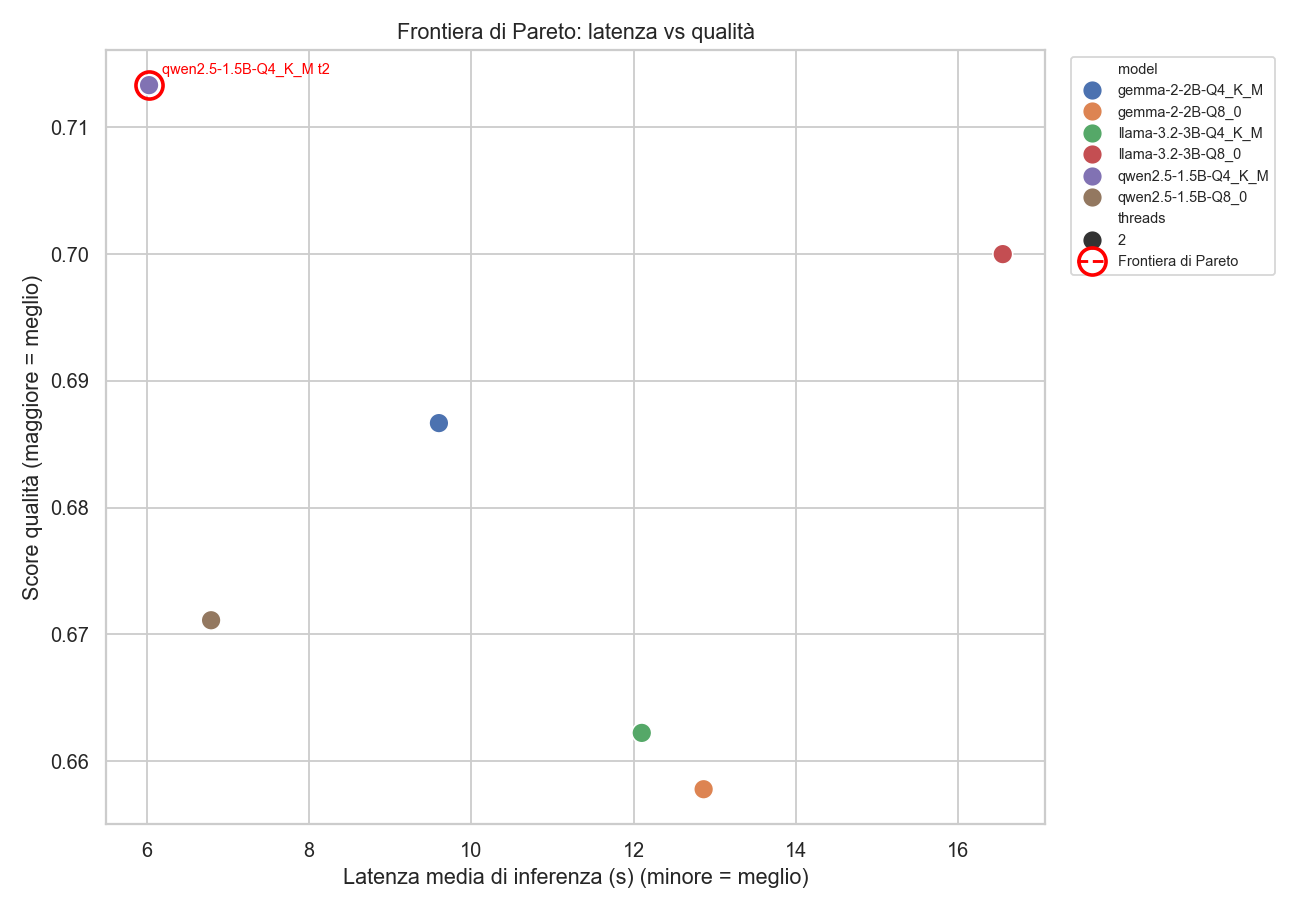
\includegraphics[width=\textwidth]{imm/pareto_latenza.png}
    \caption{Frontiera di Pareto nel piano latenza--qualità (Campagna A, i sei modelli a 2 thread).}
    \label{fig:res-pareto-lat}
\end{figure}

\subsection{Scelta del grado di parallelismo (Campagna B)}

Nella Campagna B la qualità non entra in gioco (il numero di thread non cambia le
risposte): latenza ed energia sono due \emph{costi} che il parallelismo influenza in
direzioni potenzialmente opposte. Rappresentando ciascuna configurazione nel piano
\textbf{latenza--energia} si individuano, per ogni modello, le combinazioni di thread
\emph{non dominate}. La Figura~\ref{fig:res-pareto-thread} riporta, per i sei modelli,
la traiettoria al variare dei thread (1, 2 e 4) e marca in rosso le configurazioni
dominate. Il risultato è netto: la configurazione a \textbf{4 thread è dominata in
cinque modelli su sei}, perché rispetto ai 2 thread consuma di più senza ridurre la
latenza (anzi spesso aumentandola); l'unica eccezione è qwen2.5-1.5B Q4\_K\_M, mentre per
Llama-3.2-3B Q4\_K\_M la dominanza è ancora più forte (risultano dominati sia 1 sia 4
thread, e l'unico punto sulla frontiera è quello a 2 thread). La frontiera di ciascun
modello si riduce così ai soli 1 e 2 thread: la scelta razionale è tra \textbf{1 thread}
(energia minima, ma latenza elevata) e \textbf{2 thread} (latenza minima, con un modesto
sovrapprezzo energetico), mentre i 4 thread quasi mai rappresentano un compromesso
ottimale --- una conferma \emph{senza pesi} dei 2 thread come miglior compromesso.

\begin{figure}[htbp]
    \centering
    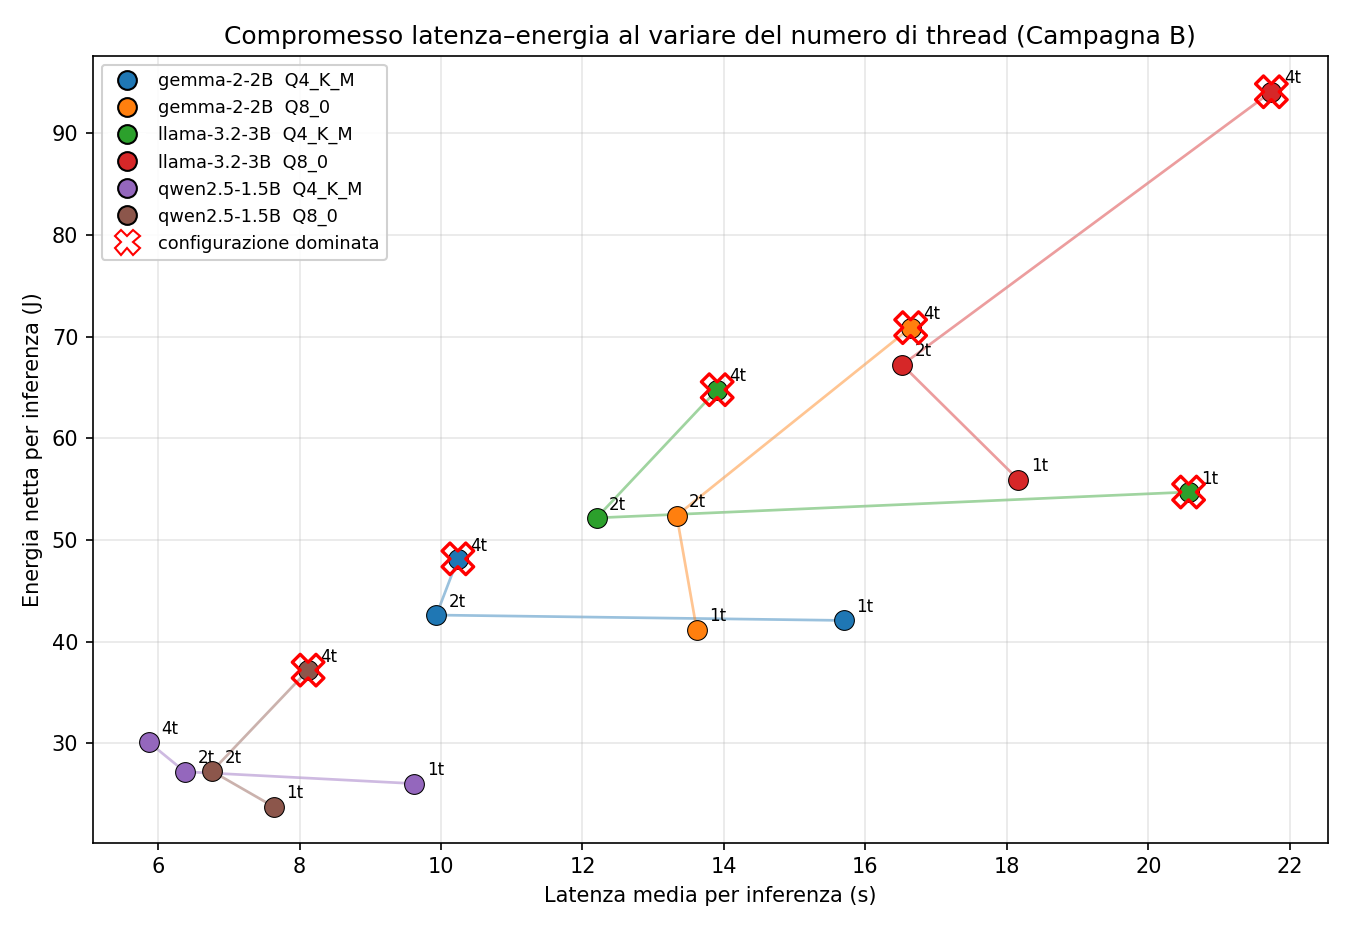
\includegraphics[width=\textwidth]{imm/pareto_lat_energia.png}
    \caption{Compromesso latenza--energia al variare del numero di thread (Campagna B):
    per ogni modello è tracciata la traiettoria a 1, 2 e 4 thread e sono marcate in rosso
    le configurazioni dominate. I 4 thread risultano dominati in cinque modelli su sei.}
    \label{fig:res-pareto-thread}
\end{figure}

\section{Sintesi: classifica complessiva}
\label{sec:composito}

Per riassumere in un unico indicatore le tre dimensioni di analisi si definisce uno
\emph{score composito}. Le tre metriche di una configurazione --- energia netta per
inferenza $E$, latenza $L$ e accuratezza media $Q$ --- hanno unità di misura e
intervalli di valori diversi; per renderle confrontabili vengono normalizzate con
una trasformazione \emph{min--max} sull'insieme delle configurazioni:
\begin{equation}
    \tilde{x} = \frac{x - x_{\min}}{x_{\max} - x_{\min}} \in [0, 1],
    \label{eq:minmax}
\end{equation}
dove $x_{\min}$ e $x_{\max}$ sono il valore minimo e massimo di quella metrica tra
tutte le configurazioni confrontate. Poiché per l'energia e la latenza sono
preferibili valori \emph{bassi}, mentre per la qualità è preferibile un valore
\emph{alto}, lo score composito $C$ è definito come media pesata in cui i termini
di energia e latenza vengono invertiti:
\begin{equation}
    C = w_E\,(1 - \tilde{E}) + w_L\,(1 - \tilde{L}) + w_Q\,\tilde{Q},
    \qquad w_E + w_L + w_Q = 1,
    \label{eq:composito}
\end{equation}
con pesi $w_E = 0{,}4$ (energia), $w_L = 0{,}2$ (latenza) e $w_Q = 0{,}4$
(qualità). A un valore di $C$ più alto corrisponde una configurazione
complessivamente migliore.

La scelta dei pesi riflette le priorità dello studio: l'\emph{efficienza
energetica} e la \emph{qualità delle risposte} sono considerate gli obiettivi
primari e ricevono quindi lo stesso peso ($0{,}4$ ciascuno), mentre alla
\emph{latenza} è attribuito un peso inferiore ($0{,}2$), essendo un requisito meno
stringente per molte applicazioni edge non strettamente interattive. Trattandosi
di una scelta soggettiva, lo score composito va inteso come una sintesi
orientativa e non come un giudizio assoluto: per questo motivo è affiancato dalla
frontiera di Pareto (Figure~\ref{fig:res-pareto-en} e~\ref{fig:res-pareto-lat}),
che individua le configurazioni ottimali \emph{senza} richiedere alcuna scelta di
pesi.

Lo score è calcolato sulle sei configurazioni della \textbf{Campagna A} (i sei
modelli a 2 thread), coerentemente con l'obiettivo di confrontare i modelli a parità
di grado di parallelismo. La Figura~\ref{fig:res-composito} riporta la relativa
classifica. La configurazione complessivamente migliore risulta
\textbf{qwen2.5-1.5B Q4\_K\_M a 2 thread} (score \textbf{1,00}), seguita da
\textbf{qwen2.5-1.5B Q8\_0} (0,67) e \textbf{gemma-2-2B Q4\_K\_M} (0,59): qwen a 4
bit ottiene il punteggio massimo perché unisce l'energia più bassa e la latenza più
bassa a una qualità competitiva --- il primato è trainato soprattutto dai vantaggi,
robusti, su energia e latenza, dato che le differenze di qualità tra i modelli di
testa rientrano nel rumore di misura ---, mentre le configurazioni Llama-3.2-3B,
penalizzate da consumo ed energia
elevati, si collocano in fondo alla classifica nonostante la buona qualità sui
task di ragionamento.

\begin{figure}[htbp]
    \centering
    
\includegraphics[width=\textwidth]{imm/ranking_composite.png}
    \caption{Classifica complessiva dei sei modelli secondo lo score composito
    (Campagna A, a 2 thread).}
    \label{fig:res-composito}
\end{figure}

\section{Comportamento termico}

Durante entrambe le campagne la temperatura del SoC è stata monitorata dopo ogni
inferenza. Grazie alla ventola di raffreddamento attiva --- e, nella Campagna B,
alle pause di raffreddamento tra le configurazioni --- la temperatura si è mantenuta
sotto la soglia di \textit{throttling} ($\sim$80--85~\textcelsius): nella Campagna A
(2 thread) il massimo è stato di \textbf{76,8}~\textcelsius, mentre nella Campagna B
i picchi si sono avuti sulle configurazioni a 4 thread, comunque contenuti intorno
agli \textbf{81}~\textcelsius\ (Figura~\ref{fig:res-termico}). In \textbf{nessuna}
delle due campagne si è verificato throttling, per cui le misure di latenza ed
energia non sono state falsate da riduzioni di frequenza indotte dal calore. Poiché in
entrambe le campagne il funzionamento è avvenuto a piena frequenza, le misure
restano inoltre \emph{direttamente confrontabili}, nonostante la Campagna B adotti
le pause di raffreddamento assenti nella Campagna A: la pausa agisce solo sulla
temperatura di picco, che al di sotto della soglia di throttling non influenza né la
latenza né l'energia.

Va tuttavia osservato che sessioni di misura molto prolungate, sommando il
riscaldamento del SoC alla sollecitazione continua in lettura della scheda microSD,
possono compromettere l'integrità dei file dei modelli memorizzati; per questo
motivo la procedura adotta la verifica di integrità all'avvio e le pause di
raffreddamento descritte nel capitolo precedente.

\begin{figure}[htbp]
    \centering
    
\includegraphics[width=\textwidth]{imm/thermal.png}
    \caption{Distribuzione della temperatura del SoC durante le inferenze della
    Campagna B, che comprende le configurazioni a 4 thread, termicamente più
    impegnative.}
    \label{fig:res-termico}
\end{figure}
